\providecommand{\main}{..}
\documentclass[\main/main.tex]{subfiles}

\begin{document}

\lesson{10}{29/10/20}
\section{Hydrodynamics and Green-Kubo relation}
We already derived the Kubo relation in the previous section: the main difference with respect what we have studied previously is that, when we consider hydrodynamic systems, we consider dependence also on \textit{spatial variables} and not only on time variables: it is the same difference between the Langevin approach (in whose context we derived the Kubo relation) and the FP approach.
In one case (L) we follow the trajectory of a single Brownian particle, while in the FP we follow the probability distribution/concentration profile for an ensemble of Brownian particles. \\

We will be dealing with the case of \textit{free particles}. In the case of hydrodynamics in general we have a conserved quantity $a$ (which could be $N,p,E,\dots$) with the corresponding density $\rho_a=\rho_a(\Vec{x},t)$; let's consider our problem in $3d$.

The current related to $\rho_a$ is called $\Vec{J}_a=\Vec{J}_a(\Vec{x},t)$. \\

We know that for a conserved quantity a \textit{continuity equation} holds:
\begin{equation}
    \derpars{t}\rho_a(\Vec{x},t)=-\Vec{\nabla}\cdot \Vec{J}_a(\Vec{x},t)
    \label{eq:cont}
\end{equation}
At this stage the continuity equation (\ref{eq:cont}) is an example of an \textit{exact microscopic law}: if the equation of motion (like the Hamilton equation) is such that a given quantity is conserved then (\ref{eq:cont}) is an exact microscopic law. \\

Let's now consider a \textbf{phenomenological (approximate) constitutive equation }: this kind of relation holds in general for \textit{weak gradients}, which means that we are in a situation of \textit{local equilibrium}, in a context where we can talk of LRT.

Being a phenomenological equation implies the use of averages:
\begin{equation}
    \left\langle\Vec{J}_{a}(\vec{x}, t)\right\rangle=-D_{a} \vec{\nabla}\left\langle\rho_{a}(\vec{x}, t)\right\rangle
    \label{eq:fl}
\end{equation}

where the proportionality constant is a generalized transport coefficient.

We can simply realize the Eq. (\ref{eq:fl}) is nothing but the Fick's law if we are dealing with number of particles as the conserved quantity and in this case the transport coefficient is the usual diffusion coefficient.

Notice that averages are involved when we write down this kind of phenomenological equations and we are dealing with non-equilibrium averages, similarly to what we already discussed.

To sum up we are considering a system mildly driven out-of-equilibrium with weak density gradients and upon this approximation we can state that the corresponding non-equilibrium current is proportional to the opposite of the gradient of the density.

The divergence of a current is zero in general to archive stationarity but at proper thermodynamic equilibrium the current itself needs to be zero: outside equilibrium the current is not zero and this is (for weak gradients) how we can compute the non-zero current in a non-equilibrium condition.

\begin{appr}
Transport coefficients can be derived also through kinetic theory e.g. for the diffusion coefficient:
\begin{equation*}
    D=\mean{v}\frac{\lambda}{3}
\end{equation*}
where $\lambda$ is the mean free path. To deppen the connection with kinetic theory see Ch.1 of the \textit{Livi, Politi} book.
\end{appr}

Putting together the constitutive equation and the continuity equation we obtain again the FP equation in the case of a free particle for the non-equilibrium average of the density associated to a conserved quantity:
\begin{equation}
    \frac{\partial\langle\rho_a(\vec{x}, t)\rangle}{\partial t}=D_a \vec{\nabla}^{2}\langle\rho_a(\vec{x}, t)\rangle
\end{equation}

When LRT holds (which is the same approximation thanks to we can write also the constitutive equation) we can say that the no-equilibrium average is proportional to equilibrium averages and in particular we can consider that:
\begin{equation}
    \mean{\rho_a(\vec{x},t)} \propto \underbrace{\mean{\rho_a(\vec{x},t')\rho_a(\vec{y},t)}_0}_{:=C(\vec{x}-\vec{y},\, t-t')}
\end{equation}

Essentially we need to  consider the A-C function of the density and the difference with what we saw in the previous lessons is that now we don't have only the time dependence but also upon spatial coordinates. The fact that the A-C function $C$ at equilibrium depends on $t-t'$ is depending on time translation invariance (energy conservation) at equilibrium, while the fact that the A-C function depends on $\vec{x}-\vec{y}$ is an \textit{assumption}: we are assuming space homogeneity in our system\footnote{Just to simplify calculations.}. \\

It's simple to realize that now we can write a FP equation for $C(\vec{x}-\vec{y},\, t-t')$\footnote{From now on we will simplify the notation writing $C(\vec{x}-\vec{y},\, t-t')=C$.}:
\begin{equation}
    \frac{\partial C}{\partial t}=D \vec{\nabla}_{\vec{x}}^{2} C
\end{equation}

Let's now consider the FT (both in space and in time) starting from the one in space (where $\vec{k}$ is the wavevector and $\int_{V}$  denotes the integral over the volume$ V $ of the system. ):
\begin{equation}
    C\left(\vec{k}, t-t^{\prime}\right)=\int_{V} d \vec{x} e^{-i \vec{k} \cdot(\vec{x}-\vec{y})} C\left(\vec{x}-\vec{y}, t-t^{\prime}\right)=
\end{equation}
exploiting the spatial homogeneity property the previous expression is independent of $\vec{y}$ and so:
\begin{equation}
    C\left(\vec{k}, t-t^{\prime}\right)=\frac{1}{V}\left\langle\rho(\vec{k}, t) \rho\left(-\vec{k}, t^{\prime}\right)\right\rangle_{0}
    \label{eq:33}
\end{equation}

The main point is that, using the LRT trick, we are now dealing with equilibrium averages.

We can now write how the FP equation looks like in FS with respect to the spatial variables:
\begin{equation}
    \frac{\partial C(\vec{k}, t)}{\partial t}=-D k^{2} C(\vec{k}, t)
\end{equation}
whose solution for $t>0$\footnote{Because we considered the initial solution at $t=0$; for negative times we can use the fact that the A-C function is even under time reversal, namely $C(\vec{k}, -t)= C(\vec{k}, t)$. For this reason the solution $\forall \,t$ is $ C(\vec{k}, t)=\mathscr{C}\exp \left(-D k^{2} |t|\right)$.} is an exponentially decaying in time, namely:
\begin{equation}
   C(\vec{k}, t)=\exp \left(-D k^{2} t\right) \underbrace{C(\vec{k}, 0)}_{:=\mathscr{C}}
\end{equation}
The property of time reversal of the (non-equilibrium average of) A-C function holds if we assume that we have invariance under mirror symmetry: $C\left(\vec{x}-\vec{y}, t\right)=C\left(\vec{y}-\vec{x}, t\right)$. From this we can derive the invariance under time reversal. \\

Once we have solved the FP equation in FS with respect to the spatial coordinates, now we perform a time FT:
\begin{align}
    C(\vec{k}, \omega) &=\int_{-\infty}^{+\infty} d t e^{-i \omega t} C(\vec{k}, t) = \int_{-\infty}^{+\infty} d t e^{-i \omega t} \mathscr{C}\exp \left(-D k^{2} |t|\right) = \\
    &\overset{(a)}{=} =\mathscr{C} \int_{0}^{+\infty} d t e^{-D k^{2} t}\left(e^{-i \omega t}+e^{i \omega t}\right) = \\
    &=\mathscr{C}\left[\frac{1}{D k^{2}+i \omega}+\frac{1}{D k^{2}-i \omega}\right] = \\
    &=\mathscr{C} \frac{2 D k^{2}}{\omega^{2}+\left(D k^{2}\right)^{2}}
\end{align}
where in (a) we separated the integral in two contributions, one for positive times and the second for negative times. The result is a Lorentzian function with width $Dk^2$.

According to LRT this is the typical frequency at which dissipation occurs and it is  also the inverse of the relaxation time to equilibrium according to the solution of the FP equation for a given $\vec{k}$ in FS. \\

At equilibrium, when $\vec{k}=0$ and I'm interested in the value of the conserved quantity averaged over the whole space, we don't have dissipation (the width of the Lorentzian is zero) and the relaxation time is infinite. Computing the limit:
\begin{equation}
   \boxed{ \lim _{k \rightarrow 0} \frac{1}{k^{2}} C(\vec{k}, \omega)=\mathscr{C} \frac{2 D}{\omega^{2}}}
   \label{eq:star}
\end{equation}

The whole point is to be able to associate the diffusion coefficient to the current- current A-C function. \\

Let's now start from the continuity equation and its FT (at first with respect to the spatial coordinates):
\begin{equation}
    \frac{\partial \rho(\vec{k}, t)}{\partial t}+i \vec{k} \cdot \vec{J}(\vec{k}, t)=0
\end{equation}
From the equilibrium average of the A-C function (\ref{eq:33}) we compute the derivatives with respect $t,t'$:
\begin{align}
    \frac{\partial}{\partial t} \frac{\partial}{\partial t^{\prime}} C\left(\vec{k}, t-t^{\prime}\right)&=\frac{1}{V}\left\langle \frac{\partial \rho(\vec{k}, t)}{\partial t} \frac{\partial \rho\left(-\vec{k}, t^{\prime}\right)}{\partial t^{\prime}}\right\rangle = \\
    &\overset{(b)}{=} \frac{1}{V} \sum_{i, j} k_{i} k_{j}\left\langle J_{i}(\vec{k}, t) J_{j}\left(-\vec{k}, t^{\prime}\right)\right\rangle_{0}
    \label{eq:miam}
\end{align}

where in (b) we explicitly write the scalar product and because of the fact that there are two such contributions the imaginary unit isn't present anymore.

Let's now consider the time FT:

\begin{equation}
    \int_{-\infty}^{+\infty} d\left(t-t^{\prime}\right) e^{-i \omega\left(t-t^{\prime}\right)} := ({\star})
\end{equation}

Let's apply the FT both to the left and right hand side of (\ref{eq:miam}):
\begin{equation}
    \omega^2 C(\vec{k},\omega)=\frac{1}{V}\int_{-\infty}^{+\infty}d(t-t')\exp{-i\omega(t-t')}\sum_i k_ik_j\mean{J_i^T(\vec{k}, t)J_j^{T}(-\vec{k},t')}_0
\end{equation}


where in the right hand side I get the correlation
function between two quantities that are essentially the \textit{total current}:
\begin{equation}
    J_{i}^{T}(t) := \lim_{k\to 0} J_{i}(\vec{k}, t)= \int_V d\vec{x}J_i(\vec{x},t)
\end{equation}
which is the integral of the current in the whole space, therefore we call it total current. \\

Let's now consider the limit of the following quantity:
\begin{align}
    \lim _{\omega \rightarrow 0} \lim _{\vec{k} \rightarrow 0} \frac{\omega^{2}}{k^{2}} C(\vec{k}, \omega)=\frac{1}{V}\int_{-\infty}^{+\infty} d(t-t')\lim_{k\to 0}\frac{\sum_{ij}k_ik_j}{k^2}\cdot\mean{J_{i}^T(t)J_{j}^T(t')}_0
\end{align}

We already assumed that our system is homogeneous in space (invariant under mirror symmetry in any direction)
 and now we will assume that the system is also \textit{isotropic}, which means that the A-C function us diagonal and so for $d$ dimension holds:
\begin{equation}
    \mean{J_{i}^T(t)J_{j}^T(t')}_0=\frac{\delta_{ij}}{d}\mean{\vec{J}^T(t)\vec{J}_j^T(t')}
\end{equation}
using the previous relation we get:

\begin{align}
     \lim _{\omega \rightarrow 0} \lim _{\vec{k} \rightarrow 0} \frac{\omega^{2}}{k^{2}} C(\vec{k}, \omega)=\frac{\hlc{yellow}{2}}{Vd}\int_{0}^{+\infty}dt \mean{\vec{J}^T(t)\vec{J}_j^T(t')}_0
     \label{eq:prev}
\end{align}

where the yellow factor is due to the fact that we were separating the contribution of positive and negative times and we also used the invariance under time reversal of the total current $\vec{J}^T(t)=\vec{J}_j^T(-t)$ so the contribution from negative times is the same of the positive times. \\

If we now multiply Eq. (\ref{eq:star}) by $\omega^2$ and then we take the zero frequency limit we get exactly the left hand side of eq. (\ref{eq:prev}).

We can conclude, thanks to (\ref{eq:star}) and (\ref{eq:prev}), that the transport/diffusion coefficient can be expressed in this way:
\begin{equation}
  \boxed{ D =\frac{1}{ V d \mathscr{C}} \lim_{\epsilon\to 0^+}\int_{0}^{+\infty} d t\exp{-\epsilon t}\left\langle\vec{J}^{T}(t) \cdot \vec{J}^{T}(0)\right\rangle_{0}}
\end{equation}
where $\mathscr{C} = C(0,0) = \int_Vd\vec{x}C(\vec{x},0)$
and this is known as the general \textit{Green-Kubo relation} dealing with a generic conserved quantity. This equation expresses a
transport coefficient $D$, associated with a density $\rho_a(\vec{x}, t)$, in terms of the time integral of
the auto-correlation function of the total current $\vec{J}^T(t)$. 

The importance of this relation is that it can be used practically in numerical simulation computing the A-C function (and so the transport coefficient of the studied system).
\paragraph{Example for $1d$ system of $N$ particles} In this example particles of mass $m$ interact through a nearest neighbour potential and so particles are arranged in lattice sites (in $1d$), defined as $ V(x_{n+1}-V(x_n))$, where the subscript $n$ labels
the lattice site and the variable $x_n$ can be read as the displacement of the nth particle with
respect to its equilibrium position, as showed in Figure \ref{fig:lattice}. If we consider PBC and if we enforce the constraint that the centre of mass velocity is null $v_{CM}=0$ one can prove that the bulk viscosity\footnote{Viscosity is the transport coefficient associated to momentum conservation, so in this example we will be interested in the momentum current-current A-C function} in the system $\eta_B$ can be computed in this way:
\begin{equation}
    \eta_B=\frac{1}{NT}\int_0^{+\infty}dt \mean{J_p(t)J_p(0)}_0
\end{equation}

where $J_p(t):=\sum_{n=1}^N F_n(t)$ is the \textit{total momentum flux}: the flux in $1d$ is the time variation of the momentum, which is the force. 

\begin{figure}[ht]
    \centering
    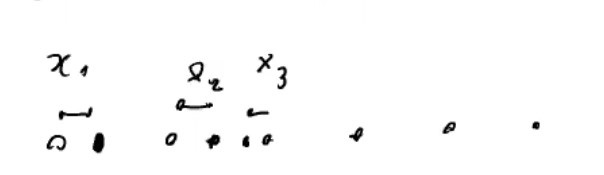
\includegraphics[width=0.6\linewidth]{Lectures/Images/latt.jpg}
    \caption{Lattice sites.}
    \label{fig:lattice}
\end{figure}

In this context the equations of motion are:
\begin{align}
    m\ddot{x}_n &=-F_n+F_{n-1} \\
    F_n &= - V'(x_{n+1}-x_{n})
\end{align}

One can use the Green-Kubo relation to compute the thermal conductivity $k$:
\begin{equation}
    \kappa=\frac{1}{N T^{2}} \int_{0}^{+\infty} d t\left\langle J_{E}(t) J_{E}(0)\right\rangle
\end{equation}
in this case the conserved quantity is energy associated to thermal conductivity as a transport coefficient (for this reason we find the energy-energy current auto-correlation function) and the \textit{total heat flux} can be computed such as:
\begin{equation}
    J_{E}(t)=\frac{1}{2} \sum_{n=1}^{N} F_{n}(t)\left(\dot{x}_{n+1}+\dot{x}_{n}\right)
\end{equation}
so the heat flux is the heat times the velocity  and one takes into account in this way that there for each particle the two different contributions from the two different neighbours.

\section{Generalized linear response functions}
We have to consider that if $h(t)$ is able to perturb its conjugated macroscopic observable $X(t)$ to which it is directly coupled, it also can influence the dynamical state of other macroscopic observables. 
More precisely, we can generalize what was discussed by introducing a perturbed Hamiltonian that depends on \textit{a set} of thermodynamic observables $X_{k}(t)$ and their conjugate (time-dependent) perturbation fields $h_{k}(t)$: therefore we will introduce different pairs of conjugated variables such that
\begin{equation}
\mathcal{H}^{\prime}=\mathcal{H}-\sum_{k} h_{k}(t) X_{k}
\end{equation}

The main difference with the case we've seen so far is that a given perturbation $h_j(t)$ can induce a response also in other non conjugated observables $X_i$ with $i\neq j$.

Similarly to what we've done in the previous lectures we will assume that the equilibrium average of all observables is zero, i.e. $\mean{X_k}_0 = 0\,\forall k$ and the definition of the response function is through the following equation, where we are interested in computing thee non-equilibrium average through a convolution of a response function that takes into account the response of the variable $X_i$ to the perturbation $h_j(t)$:

\begin{equation}
    \left\langle X_{i}(t)\right\rangle=\int_{-\infty}^{+\infty} d t^{\prime} \Xi_{i j}\left(t-t^{\prime}\right) h_{j}\left(t^{\prime}\right)
\end{equation}
The order in which we write the indexes in the response function is important because $\Xi_{ij}$ denotes the response of variable $X_i$ to the perturbation $h_j(t)$ and we know, similarly to what we saw in the last lectures, that we can express the response function as:
\begin{equation}
    \Xi_{i j}(t)=-\beta \theta(t) \frac{d}{d t}\left\langle X_{i}(t) X_{j}(0)\right\rangle_{0}
\end{equation}
In FS (frequency domain) the definition of response function becomes:
\begin{equation}
    \mean{X_i(\omega)}=\Xi_{ij}(\omega)h_j(\omega)
\end{equation}
where 
\begin{equation}
    \Xi_{i j}(\omega)=-\beta \int_{-\infty}^{+\infty} \frac{d \omega^{\prime}}{2 \pi} \theta\left(\omega-\omega^{\prime}\right)\left(i \omega^{\prime}\right) C_{i j}\left(\omega^{\prime}\right)
\end{equation}

and $C_{ij}(\omega)$ is a quantity which is analogous to the power spectrum but for two different observables; it is defined as the FT of the equilibrium average correlation function:
\begin{align}
    C_{ij}(\omega)&=\int_{-\infty}^{+\infty} dt \exp{-i\omega t}\mean{X_i(t)X_j(0)}_0 = \\
    &=\lim_{T\to\infty}\frac{1}{T}\mean{|X_{i,T}^*(\omega)X_{j,T}|}_0
\end{align}
where the order of the indexes is important because in this case the perturbation is $j$ while the responding variable at later time is $i$ and $C_{ij}(\omega)\geq 0$ is a real positive number. \\

The F-D relation holds in a very similar way to the previous one such that 
\begin{equation}
    \Xi_{i j}^{I}(\omega)=-\frac{\beta \omega}{2} C_{i j}(\omega); \quad \Xi_{i j}^{R}(\omega)={PV} \left[\int_{-\infty}^{+\infty} \frac{d \omega^{\prime}}{\pi} \frac{1}{\omega^{\prime}-\omega} \Xi_{i j}^{I}\left(\omega^{\prime}\right)\right]
\end{equation}

In this way we extended what we have learnt in the previous lessons extending it to the case of the action of a perturbation inducing a response for a variable that is not the variable conjugated to it (in a thermodynamic sense). \\

If we chose, going back to the simplest case, the step-wise perturbation which is switched off instantaneously at $t=0$ (which is represented in Figure \ref{fig:h}), namely
\begin{equation}
    h_i(t)=h\theta(-t)
\end{equation}
we recover a simple way to express the non-equilibrium average related to an equilibrium correlation function between the two variables $X_i,X_j$
\begin{equation}
    \mean{X_i(t)}=\beta h\mean{X_i(t)X_j(0)}_0 
    \label{eq:onsager}
\end{equation}

\begin{figure}[ht]
    \centering
    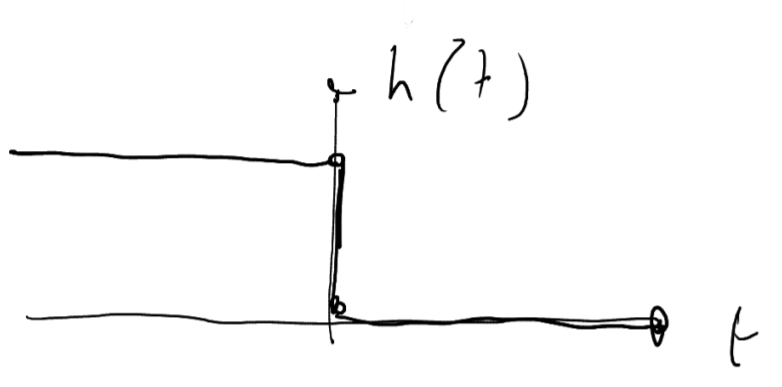
\includegraphics[width=0.5\linewidth]{Lectures/Images/h.png}
    \caption{Step-wise perturbation $h(t)$.}
    \label{fig:h}
\end{figure}

where on the left hand side we can find the non-equilibrium relaxation to the equilibrium value while on the right hand side we find the equilibrium decay of the correlation function. 

Again, how a given observable $X_i$ relaxes to equilibrium after a perturbation induced by the field coupled conjugated a to different observable $X_j$ is essentially controlled by the properties of the equilibrium auto-correlation function between the two variables $X_i, X_j$, \textit{always in the limit of small perturbation}. \\

It is important to observe that historically relation (\ref{eq:onsager}) was proposed first by Onsager and it is actually known as the \textbf{Onsager regression relation}.

\textit{Regression} because it is not obvious the point that, if we perturb the field conjugated to some observable $X_j$, also another observable like $X_i$ will respond to this perturbation.

Another way to state the properties encoded in equation (\ref{eq:onsager}) is to say that if we observe some fluctuations/decay with time in a system we cannot tell whether it is a non-equilibrium relaxation or it is just the decay of some equilibrium fluctuations when the perturbations are small.

\subsubsection{Time reversal properties of $\Xi_{ij}(t)$}
Let's introduce a time-reversal
operator $\mathcal{T}$ whose action applies to the phase–space points $\{q_k(t),p_k(t)\}_{t=0,T}\,\,$\footnote{Which are trajectories solving the Hamilton equations with initial conditions given by the values at zero time $(q_k(0),p_k(0))$.} as:

\begin{equation}
   \mathcal{T}\left(q_{k}(t), p_{k}(t)\right)=\left(q_{k}(t),-p_{k}(t)\right)
\end{equation}

The point about reversibility property (which corresponds to detailed balance in stochastic processes) is that if $(q_k(t),p_k(t))$ is a trajectory with initial conditions $(q_k(0),p_k(0))$ then the time-reversed trajectory, which can be formally archived by using the time-reversal operator, it is also a solution with initial conditions $\mathcal{T}(q_k(0),p_k(0))$.

\begin{figure}[ht]
    \centering
    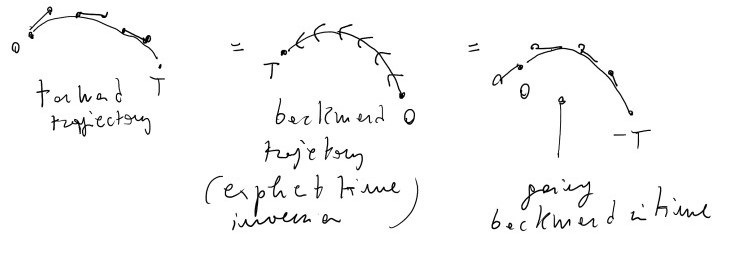
\includegraphics[width=0.7\linewidth]{Lectures/Images/prova.jpg}
    \caption{Differences between forward, backward and time-reversed trajectories. The arrows indicate the momenta's direction.}
    \label{fig:my_label}
\end{figure}

So with \textit{time-reversed trajectory} we mean that the trajectory starts from the same coordinate as the forward trajectory but then going backwards in time. This fact is important because we will now assume that my observables $X_i$ are eigenfunctions of the time-reversal operator $\mathcal{T}$: which are the eigenvalues?

Considering a time reversed trajectory it's like going backwards in time and in general our observable $X_i$ is a function of the coordinates, so applying $\mathcal{T}$ to $X_i$ or to its coordinates is the same:
\begin{align}
    X_i(-t)=\mathcal{T}X_i(t)&=X_i(\mathcal{T}(q_k(t),p_k(t)))= \\
    &=X_i(q_k(t),-p_k(t))= \\
    &=\tau_iX_i(t)
\end{align}
where $\tau_i$ is the eigenvalue of our observable $X_i$ with respect to time reversal operator and we can have \textit{even} or \textit{odd} observables upon time reversal, $\tau_i=\pm 1$.

On the other hand, applying the time-reversal operator to the Hamiltonian (which is invariant under time reversal, $\mathcal{H}=\mathcal{T}\mathcal{H}$) it means that at equilibrium the Boltzmann distribution $\exp{-\beta \mathcal{H}}$ is the same for the forward and time-reversed trajectories. \\

Let's now compute the equilibrium correlation function between two different observables $\mean{X_i(t)X_j(0)}_0$.

We consider this correlation function having in mind the forward trajectories, meaning that we sample the forward trajectories according to Boltzmann distribution: we will switch considering time-reversed trajectories but since the Boltzmann distribution is the same we can state that an equilibrium average performed over a Boltzmann distribution for the time-reversed trajectory needs to give the same result. Using the action of the $\mathcal{T}$ operator:
\begin{align}
    \mean{X_i(t)X_j(0)}_0 &=\mean{\mathcal{T}X_i(-t)\mathcal{T}X_j(0)}_0 =\\ &\overset{(a)}{=} \tau_i\tau_j\mean{X_i(-t)X_j(0)}_0 = \\
    &\overset{(b)}{=}\tau_i\tau_j\mean{X_j(t)X_i(0)}_0
\end{align}

where we can state that the two averages are the same because we are considering on the left hand side an average over forward trajectories using the Boltzmann distribution and on the right hand side an average over time-reversed trajectories using the Boltzmann distribution again and which is invariant under time reversal. In (a) then we used the fact that $X_i,X_j$ are eigenfunctions of the time-reversal operator, while in (b) the time translation invariance adding $t$ to both arguments.

We can conclude that the correlation functions of observables with the same parity with
respect to time reversal are even functions of time, while those of observables with different
parity are odd functions of time. This result has important consequences for the properties
of the response function, that, for $t > 0$, can be rewritten as (switching $i$ with $j$):
\begin{equation}
 \Xi_{i j}(t)=-\beta \theta(t) \frac{d}{d t}\left\langle X_{i}(t) X_{j}(0)\right\rangle_{0}=-\beta \tau_{i} \tau_{j} \theta(t) \frac{d}{d t}\left\langle X_{j}(t) X_{i}(0)\right\rangle_{0}   
\end{equation}
We said at the beginning of this part that the order in which I write the indexes in the response function is important: for example $\Xi_{ij}(t)$ is the response of $i$ to $j$ but are there any relations with the response function describing how $j$ response to $i$? The connection is related to the time-reversal invariance properties of the two observables:

\begin{equation}
    \boxed{\Xi_{ij}(t)=\tau_i\tau_j\Xi_{ji}(t)}
    \label{eq:scambio}
\end{equation}
Equation (\ref{eq:scambio}) tells us that the response function may be symmetric in the case we are dealing with two observables with the same parity under time reversal or may be anti-symmetric in the case we are dealing with two observables with different parities under time reversal.

\section{Entropy Production, Fluxes, and Thermodynamic Forces (Affinities)}
In this section we will start to introduce how we can merge the Onsager theory used to describe how a given observable respond to the perturbation coupled to another observable and the context of entropy production. \\

Let's start recalling the \textbf{second law of thermodynamics}: \textit{for isolated systems entropy always increases} ($dS\geq 0$) \textit{and in particular, in out-of-equilibrium (or irreversible) processes} $dS>0$ \textit{and so entropy is produced, whereas in equilibrium the entropy of an isolated system doesn't change ($dS=0$) and $S$ is maximum at equilibrium}.\footnote{Remember that entropy is an extensive variable.} \\

Let's now consider the whole system (the \textit{universe}) as divided in two subsystems: 
\begin{center}
    universe = system + reservoir
\end{center}

We will refer to the total variation of entropy of the universe with $d\mathbb{S}$ and we will assume that in this
universe the total variation of entropy can be written as:
\begin{align}
    d \mathbb{S}=d S+d S_{r}
\end{align}
i.e., it is the sum of the variation of entropy in the system, $dS$, and in the reservoir, $dS_r$.

The second law implies then that $d\mathbb{S}\geq 0$: the other two variations $dS,dS_r$ could be negative by themselves (but not all of them at the same time). For example we can deal with an \textit{adiabatic process} where, by definition, the system doesn't exchange heat with the reservoir such that $dS_r=0$ (and $dQ=0$) and the second law can be stated as $dS=d\mathbb{S}\geq 0$ and the entropy of the universe increases as the entropy of the system.

A second example can be explained with an \textit{isothermal process}: in this case some heat $dQ>0$ is exchanged\footnote{We will use the sign convention according to which $dQ$ is positive when the heat is absorbed by the system and lost by the reservoir.} between the system and the reservoir. In this case the entropy variation in the reservoir is:
\begin{equation}
    dS_r=-\frac{dQ}{dt}
    \label{eq:2law}
\end{equation}
where the '-' sign is due to the fact that the heat is \textit{lost} by the reservoir and according to the second laww we can state that:
\begin{equation}
    dS=d\mathbb{S}-dS_r\overset{(\ref{eq:2law})}{\geq} 0 + \frac{dQ}{dt} \quad \implies \quad \boxed{dS \geq \frac{dQ}{dt}}
\end{equation}
Again, if we are dealing with equilibrium processes then $dS=dQ/dt$, where $Q$ is the heat absorbed by the system. \\

The key point is that we have a relation between \textit{entropy production} and \textit{thermodynamic forces}, which cause entropy production.

Essentially, saying that the system is out-of-equilibrium implies to say that there is a non zero thermodynamic force acting into the system that will try to restore the equilibrium in the system and in doing so it will produce entropy.

Let's say that our (system) entropy is a function of several extensive thermodynamic observables $X_i$, namely
\begin{equation}
    S=S(\{X_i\})
\end{equation}

Due to their extensive character, we can assume that a given value $\mathbb{X}_{i}$ taken in our universe by one of these observables has to be the sum of the values taken by this observable in the system, $X_{i},$ and in the reservoir, $X_{i}^{(r)},$ that is,
\begin{align}
  \mathbb{X}_{i}=X_{i}+X_{i}^{(r)}  
\end{align}

An important point is that $X_i$ is a \textit{conserved quantity} and this implies that the variation in the universe is zero and therefore $d\mathbb{X}_i=0\,\,\, \implies\,\,\, \hlc{yellow}{dX_i=-dX_i^{(r)}}$.

On the other hand the \textit{thermodynamic force} for the universe is defined in the following way:
\begin{equation}
    \left.\mathbb{F}_{i} \equiv\left(\frac{\partial \mathbb{S}}{\partial X_{i}}\right)\right|_{X_{i}=\mathbb{X}_{i}}=\frac{\partial S}{\partial X_{i}}\hlc{yellow}{-}\frac{\partial S_{r}}{\partial X_{i}^{(r)}} := F_{i}-F_{i}^{(r)}
\end{equation}

We are allowed to use this definition because (-)entropy is the thermodynamic potential for an isolated system and therefore if we know how the universe entropy depends on the system variables $X_i$ then we can define a thermodynamic force. The '-' sign is due to the fact that we are using the highlighted relation, while $F_i$ is the thermodynamic force in the system and $F_i^{(r)}$ is the force contribution coming from the reservoir. The thermodynamic force of the universe $\mathbb{F}$ is also called \textit{affinity}. \\

What happens at equilibrium is that $d\mathbb{S}=0$ and so $\mathbb{S}$ is at its maximum value. Therefore this implies that the corresponding affinity $\mathbb{F_i}=0\,\, \forall\, i$. Let us assume for simplicity that the values of different observables at equilibrium (denoted with a $^*$) are all equal to zero, $X_i^*=0\,\,\forall \,i$. On the other hand if $\mathbb{F}_i\neq 0$ then we deal with irreversible processes that set up in order to restore equilibrium. \\

We can exemplify our previous considerations about a system in out-of-equilibrium conditions by first recalling that typical examples of extensive thermodynamic observables are the internal energy $U,$ the volume $V,$ and the number of particles $N_{j}$ of the species $j$ contained in the system. The Gibbs relation
\begin{equation}
T d S=d U+P d V-\sum_{j} \mu_{j} d N_{j} 
\label{eq:gibbs}
\end{equation}

provides us with the functional dependence of $S$ on these extensive observables, where $T$ is
the absolute temperature, $P$ is the pressure, and$\mu_j$ is the chemical potential of particles of
species $j$.

Using relation (\ref{eq:gibbs}) implies the assumption of \textit{local equilibrium}: we are trying to describe a situation in which there is globally no equilibrium (because we have some thermodynamic forces different from zero) but the fact that we are using this relation assuming that at least locally we can define the variation of entropy, this implies that at least locally we are assuming equilibrium (or we are dealing, in the thermodynamic language, with \textit{quasi-reversible processes}\footnote{Which is more correct because talking about local equilibrium implies the presence of space (variation with space) and in what we will do now there is no spatial variables, therefore the correct statement is talking about quasi-reversible processes.}).


We assume that such a functional dependence is valid also for the above described out-of-equilibrium conditions. For instance, we can still define the absolute temperature of the system and of the reservoir (or of the two subsystems) by the expression
\begin{equation}
    \left(\frac{\partial S}{\partial U}\right)_{V, N_{j}}=\frac{1}{T}
\end{equation}

and, analogously, the pressure and chemical potentials by the 
\begin{equation}
    \left(\frac{\partial S}{\partial V}\right)_{U, N_{j}}=\frac{P}{T}, \quad\left(\frac{\partial S}{\partial N_{j}}\right)_{U, V}=-\frac{\mu_{j}}{T}
\end{equation}

At this point let's compute the affinities with respect the variation of a quantity:
\begin{equation}
    \mathbb{F}_{U}=\frac{1}{T}-\frac{1}{T_{r}}, \quad \mathbb{F}_{V}=\frac{P}{T}-\frac{P_{r}}{T_{r}}, \quad \mathbb{F}_{N_{j}}=-\frac{\mu_{j}}{T}+\frac{\mu_{j}^{(r)}}{T_{r}}
\end{equation}

At equilibrium we get the well known result for which $\mathbb{F}_U=\mathbb{F}_V=\mathbb{F}_{N_j} = 0 \,\,\, \implies \,\,\, T,P,\mu_i$ needs to be the same in the system and in the reservoir.

If e.g. $T_r\neq T$ we have that heat flows from/to the reservoir, to/from the system in order to restore an equilibrium situation in which the two temperatures are the same; this implies also that $U$ changes in the system.

In general we introduce the concept of \textit{flux} when we deal with the change in time of some observables:

\begin{equation}
    J_i=\frac{d X_i}{dt}
\end{equation}
The presence of a non-zero flux is related to a non-equilibrium situation in which there is a non-zero affinity: $\mathbb{F}_i \neq 0 \implies J_i \neq 0$
(which is a non-equilibrium situation).

This it will start an entropy production and if we consider the previous equation we can define the rate of entropy as:
\begin{equation}
    \frac{d \mathbb{S}}{d t}=\sum_{i}\left(\hlc{yellow}{\frac{\partial S}{\partial X_{i}}-\frac{\partial S_{r}}{\partial X_{i}^{(r)}}}\right) \hlc{green}{\frac{d X_{i}}{d t}}=\sum_{i} \hlc{yellow}{\mathbb{F}_{i}} \hlc{green}{J_{i}} \geq 0
    \label{eq:entropy}
\end{equation}
In the end Equation (\ref{eq:entropy}) is the universe production rate. At equilibrium $J_i=0,\mathbb{F}_i=0$ and $d\mathbb{S}/dt=0$: entropy doesn't change; on the other hand at non-equilibrium $\mathbb{F}_i, J_i \neq 0, d\mathbb{S}>0$.

There real condition for equilibrium is having zero affinities and there may be particular situations in which non-zero fluxed may be present at  equilibrium. From the equation for the entropy production rate we just need that affinity be zero in order for the entropy production to be zero. \\

Since our universe is isolated, the second principle of thermodynamics states that in out-of-equilibrium conditions the total entropy has to increase, namely,
$$
\frac{d \mathbb{S}}{d t}=\sum_{i} \mathbb{F}_{i} J_{i} \geq 0
$$
and it vanishes only when all affinities and the corresponding fluxes vanish, i.e., at thermodynamic equilibrium.\footnote{There are peculiar situations in coupled transport processes, where, as a consequence of
symmetries, a flux can be made to vanish by applying suitable, non-vanishing affinities, although the system is
kept in stationary out-of-equilibrium conditions.}

\end{document}